\documentclass[12pt]{article}
\usepackage{amsmath}
\usepackage{graphicx}
\usepackage{hyperref}
\usepackage{listings}
\usepackage{color}
\usepackage{pythonhighlight}

\title{Operating System Course Report - First Half of the Semester}
\author{B class}
\date{\today}

\begin{document}

\maketitle
\newpage

\tableofcontents
\newpage

\section{Introduction}
This report summarizes the topics covered during the first half of the Operating System course. It includes theoretical concepts, practical implementations, and assignments. The course focuses on the fundamentals of operating systems, including system architecture, process management, CPU scheduling, and deadlock handling.

\section{Course Overview}
\subsection{Objectives}
The main objectives of this course are:
\begin{itemize}
    \item To understand the basic components and architecture of a computer system.
    \item To learn process management, scheduling, and inter-process communication.
    \item To explore file systems, input/output management, and virtualization.
    \item To study the prevention and handling of deadlocks in operating systems.
\end{itemize}

\subsection{Course Structure}
The course is divided into two halves. This report focuses on the first half, which covers:
\begin{itemize}
    \item Basic Concepts and Components of Computer Systems
    \item System Performance and Metrics
    \item System Architecture of Computer Systems
    \item Process Description and Control
    \item Scheduling Algorithms
    \item Process Creation and Termination
    \item Introduction to Threads
    \item File Systems
    \item Input and Output Management
    \item Deadlock Introduction and Prevention
    \item User Interface Management
    \item Virtualization in Operating Systems
\end{itemize}

\section{Topics Covered}

\subsection{Basic Concepts and Components of Computer Systems}
This section explains the fundamental components that make up a computer system, including the CPU, memory, storage, and input/output devices.

\subsection{System Performance and Metrics}
This section introduces various system performance metrics used to measure the efficiency of a computer system, including throughput, response time, and utilization.

\subsection{System Architecture of Computer Systems}
Describes the architecture of modern computer systems, focusing on the interaction between hardware and the operating system.

\subsection{Process Description and Control}
Processes are a central concept in operating systems. This section covers:
\begin{itemize}
    \item Process states and state transitions
    \item Process control block (PCB)
    \item Context switching
\end{itemize}

\subsection{Scheduling Algorithms}
This section covers:
\begin{itemize}
    \item First-Come, First-Served (FCFS)
    \item Shortest Job Next (SJN)
    \item Round Robin (RR)
\end{itemize}
It explains how these algorithms are used to allocate CPU time to processes.

\subsection{Process Creation and Termination}
Details how processes are created and terminated by the operating system, including:
\begin{itemize}
    \item Process spawning
    \item Process termination conditions
\end{itemize}

\subsection{Introduction to Threads}
This section introduces the concept of threads and their relation to processes, covering:
\begin{itemize}
    \item Single-threaded vs. multi-threaded processes
    \item Benefits of multithreading
\end{itemize}

\begin{figure}[h]
    \centering
    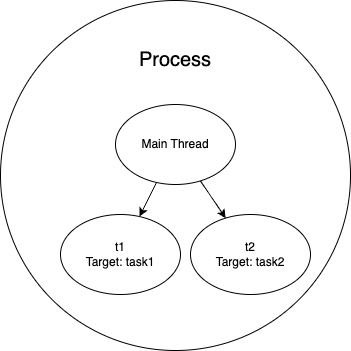
\includegraphics[width=0.5\textwidth]{/Users/khawaritzmi/Unhas/os_report_mid2024/b_class/asset/example.png}  % Sesuaikan nama file dan ukurannya
    \caption{Ini adalah gambar contoh dari multithreading.}
    \label{fig:contoh_gambar}
\end{figure}

Seperti yang terlihat pada Gambar \ref{fig:contoh_gambar}, inilah cara menambahkan gambar dengan keterangan.

\subsection{File Systems}
File systems provide a way for the operating system to store, retrieve, and manage data. This section explains:
\begin{itemize}
    \item File system structure
    \item File access methods
    \item Directory management
\end{itemize}

\subsection{Input and Output Management}

\subsubsection{Interrupt Driven I/O}
   \begin{itemize}
    \item Metode di mana perangkat I/O mengirimkan sinyal interupsi ke CPU
    saat siap melakukan transfer data. Berbeda dengan polled I/O yang mengharuskan CPU secara terus-menerus memeriksa status perangkat, dalam interrupt-driven I/O, CPU dapat fokus pada tugas lain hingga diinterupsi oleh perangkat I/O.
    \item Prinsip mekanisme transfer data pada interrupt-driven I/O sama dengan programmed I/O, yaitu CPU tetap mempertukarkan data dengan device I/O melalui beberapa register CPU. Maka antarmuka I/O menyediakan control, status, dan port data. Perbedaan yang prinsip adalah siapa yang bertanggung jawab untuk berinisiatif melakukan transfer data. Pada programmed I/O tanggung jawabnya ada pada CPU. Dengan kata lain, program I/O harus sering melakukan pemeriksaan (scan) status device I/O untuk menentukan apakah device siap melakukan transfer data.Pada interrupt-driven I/O, data transfer dimulai (atasinisiatif) device I/O, yang menggunakan mekanisme interupsi untuk memberitahukan CPU tentang kesiapannya. Mekanisme ini menghilangkan beban scanning status. Device I/O juga dapat menggunakan mekanisme interupsi untuk keperluan yang lain. Sebagai contoh untuk menarik perhatian CPU pada saat terjadi kesalahan/ kerusakkan, atau untuk menunjukkan selesainya operasi lokal.\\
    Tanpa memperhatikan tipenya, apabila menerima interupsi, CPU akan:
\begin{enumerate}
    \item Menagguhkan eksekusi program yang sedang berlangsung.
    \item Menyimpan statusnya.
    \item Melompat ke interrupt service routine (ISR).
    \item Kembali untuk melanjutkan eksekusi program yang diinterupsi.
\end{enumerate}
\end{itemize}
\subsubsection{Jenis Interupsi}
\begin{enumerate}
    \item Maskable interupts.
    \item Non-Maskable interrupts.
\end{enumerate}
\subsubsection{Struktur interupsi pada prosesor}
\begin{enumerate}
    \item Interupsi maskable dan nonmaskable dengan jalur terpisah.
\item Interupsi maskable dan nonmaskable dengan jalur bersama.\\
    Pola pertama berbasis pada dua jalur permintaan interupsi (interrupt request) yang terpisah, satu untuk interupsi maskable (INTREQ) dan satu lagi untuk nonmaskable (NMINT). Jalur INTERQ biasanya berpasangan dengan jalur interrupt acknowledge (INTACK). Melalui jalur ini CPU menjawab penerimaan permintaan nterupsi dan menginstrusksikan device I/O untuk meletakkan kode alamat ke bus data. Kode alamat menunjukkan CPU ke ISR yang mentansfer data atau melakukan pelayanan yang lainya atas nama device I/O. INTERQ dan INTACK dapat dipandang sebagai pasangan jalurjabat tangan (handshaking).Beberapa CPU tidak menyediakan sinyal jawanan interupsi pada jalur yang terpisah, tetapi melakukan enscodesiklus ini pada jalur status. Dalam kasus ini sinyal INTACKdiperoleh dengan cara mengkode jalur status CPU. Interupsi non maskable tidak memerlukan acknowledge karena interupsi ini selalu diterima dan karena tidak ada kode alamat yang diberikan secara eksternal. Dengan demikian tidak diperlukan jalur acknowledge untuk interupsi ini. Contoh prosesor yang menggunakan pola ini adalah 8086 dan 8088.
\end{enumerate}
\subsubsection{Pemrosesan Interupsi}
\begin{enumerate}
    \item Menangguhkan eksekusi program.
    \item Menyimpan status program (context).
    \item Melompat ke Interrupt Service Routine (ISR).
    \item embali ke program yang diinterupsi.
\end{enumerate}
\subsubsection{Klasifikasi Perangkat I/O}
\begin{itemize}
    \item Sifat aliran datanya
\begin{enumerate}
    \item Perangkat berorientasi blok \\
    Yaitu menyimpan, menerima, dan mengirim informasi sebagai blok-blok berukuran tetap yang berukuran 128 sampai 1024 byte dan memiliki alamat tersendiri, sehingga memungkinkan membaca atau menulis blok-blok secara independen (mandiri), yaitu dapat membaca atau menulis sembarang blok tanpa harus melewati blok-blok lain. Contoh : disk,tape,CD ROM,optical disk.
    \item Perangkat berorientasi aliran karakter \\
    Perangkat yang menerima, dan mengirimkan aliran karakter tanpa membentuk suatu struktur blok. Contoh : terminal, line printer, pita kertas, kartu-kartu berlubang, interface jaringan, mouse.
\end{enumerate}
\end{itemize}
\begin{itemize}
    \item Sasaran komunikasi 
\begin{enumerate}
    \item Perangkat yang terbaca oleh manusia \\
    Perangkat yang digunakan untuk berkomunikasi dengan manusia. 
    Contoh : VDT (video display terminal) : monitor, keyboard, mouse.
    \item Perangkat yang terbaca oleh mesin 
    Perangkat yang digunakan untuk berkomunikasi dengan perangkat elektronik. Contoh : Disk dan tape, sensor, controller.
    \item perangkat komunikasi\\
    Perangkat yang digunakan untuk komunikasi dengan perangkat jarak jauh. Contoh : Modem
\end{enumerate}
\end{itemize}
\subsubsection{Prinsip Manajemen Perangkat I/O}
\begin{itemize}
    \item Terdapat dua sasaran perancangan I/O
\begin{enumerate}
    \item Efisiensi \\
    Aspek penting karena operasi I/O sering menimbulkan bottleneck.
    \item Generalitas(device independence) \\
    Manajemen perangkat I/O selain berkaitan dengan simplisitas dan bebas kesalahan, juga menangani perangkat secara seragam baik dari cara proses memandang maupun cara sistem operasi mengelola perangkat dan operasi I/O.
\end{enumerate}
\end{itemize}
\subsubsection{Masalah-Masalah Manajemen I/O}
\begin{itemize}
    \item Penamaan yang seragam (uniform naming) \\
    Nama berkas atau perangkat adalah string atau integer, tidak bergantung pada perangkat sama sekali. 
    \item Penanganan kesalahan(errorhandling)\\
    Umumnya penanganan kesalahan ditangani sedekat mungkin dengan perangkat keras.
    \item Transfer sinkron vs asinkron \\
    Kebanyakan I/O adalah asinkron. Pemroses memulai transfer serta mengabaikan untuk melakukan kerja lain sampai interupsi tiba. Program pemakai sangat lebih mudah ditulis jika operasi I/O berorientasi blok. Setelah perintah read, program kemudian ditunda secara otomatis sampai data tersedia di buffer.
    \item Sharable vs dedicated \\
    Beberapa perangkat dapat dipakai bersama seperti disk, tapi ada juga perangkat yang hanya satu pemakai yang dibolehkan memakai pada satu saat. Contoh : printer
\end{itemize}
\subsubsection{Direct Memory Access}
Dirrect Memory Acces atau DMA merupakan suatu alat pengendali khusus yang disediakan untuk memungkinkan transfer blok data langsung antar perangkat eksternal dan memori utama, tanpa interversi terus menerus dari prosesor. \\
\begin{figure}[h]
    \centering
    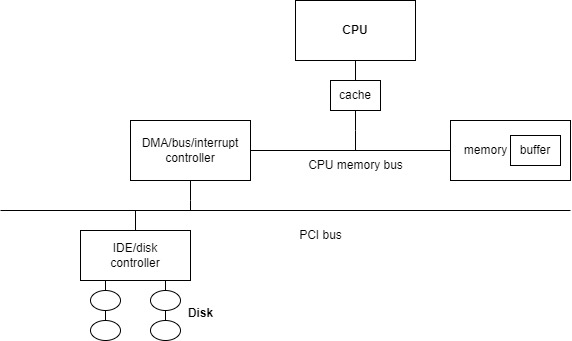
\includegraphics[width=0.80\linewidth]{b_class/asset/I_O.jpg}
    \caption{Struktur Modul I/O}
    \label{fig:enter-label}
\end{figure}
Penjelasan :
\begin{itemize}
    \item CPU Mengatur Pekerjaan
    Saat CPU memulai pekerjaan, CPU ingin memindahkan data dari disk (penyimpanan) ke RAM (memori). Untuk melakukan ini, CPU akan memberi perintah ke DMA Controller. DMA berfungsi membantu CPU agar tidak terlalu sibuk.
    \item DMA Controller Beraksi
    Setelah mendapat perintah, DMA controller mengambil alih pekerjaan untuk sementara. Dia akan membuat jalur khusus agar data dari disk bisa langsung masuk ke memori tanpa harus melalui CPU. Hal ini dilakukan agar CPU bisa tetap fokus pada tugas lain dan tidak perlu bolak-balik mengurus transfer data.
    \item Transfer Data
    DMA controller menggunakan PCI bus untuk memindahkan data dari disk ke RAM dengan menggunakan bantuan jalur-jalur khusus yang sudah ada. Dalam perjalanan ini, Pada transfer data terdapat buffer yang berfungsi sebagai tempat persinggahan sementara. Buffer menampung data sementara sebelum data benar-benar sampai ke RAM.
    \item Pemberitahuan ke CPU
    Setelah semua data berhasil dipindahkan ke RAM, DMA controller akan memberi tahu CPU dengan "sinyal interupsi." \\
    Inti dari diagram ini adalah menunjukkan bagaimana sistem komputer bisa bekerja lebih efisien menggunakan DMA. Dengan menggunakan DMA controller, CPU tidak perlu sibuk mengurus transfer data. CPU cukup memberi perintah sekali, lalu DMA yang akan menangani semua proses transfer. Hasilnya, Komputer bekerja lebih cepat dan efisien karena CPU bisa mengerjakan tugas lain tanpa terhambat.
\end{itemize}

\subsubsection{Metode DMA Dalam Mentransfer Data}
\begin{itemize}
    \item Metode HALT atau BurstMode DMA
    \item Mengikut sertakan pengendali DMA \\
    Pada dasarnya DMA mempunyai dua metode yang berbeda dalam mentransfer data, Metode yang pertama ialah metode yang sangat baku dan sederhana disebut HALT, atau BurstMode DMA, karena pengendali DMA memegang control dari system bus dan mentransfer semua blok data atau dari memori pada single burst. Selagi transfer masih dalam proses, system mikroprosessor di-setidle, tidak melakukan intruksi operasi untuk menjaga internal register. Tipe operasi DMA seperti ini ada pada kebanyakan komputer. Metode yang kedua adalah mengikut sertakan pengendali DMA untuk memegang control dari system bus untuk jangka waktu yang lebih pendek pada periode dimana mikroprosessor sibuk dengan operasi internal dan tidak membutuhkan akses ke system bus. Metode DMA ini disebut dengan cycle stealing mode. Cycle stealing mode DMA lebih kompleks untuk diimplementasikan dibandingkan HALT DMA, karena pengendali DMA harus mempunyai kepintaran untuk merasakan waktu pada saat sistem bus terbuka.
\end{itemize}

\subsubsection{Referensi}
\begin{itemize}
    \item Dancok, D. C. (2024, Mei 23). manajemen I-O. Retrieved from scribd.com: https://www.scribd.com/document/735310900/3-Manajemen-I-O 
\end{itemize}

\subsection{Deadlock Introduction and Prevention}
Explores the concept of deadlocks and methods for preventing them:
\begin{itemize}
    \item Deadlock conditions
    \item Deadlock prevention techniques
\end{itemize}

\subsection{User Interface Management}
This section discusses the role of the operating system in managing the user interface. Topics covered include:
\begin{itemize}
    \item Graphical User Interface (GUI)
    \item Command-Line Interface (CLI)
    \item Interaction between the user and the operating system
\end{itemize}

\subsection{Virtualization in Operating Systems}
Virtualization allows multiple operating systems to run concurrently on a single physical machine. This section explores:
\begin{itemize}
    \item Concept of virtualization
    \item Hypervisors and their types
    \item Benefits of virtualization in modern computing
\end{itemize}

\section{Assignments and Practical Work}
\subsection{Assignment 1: Process Scheduling}
Students were tasked with implementing various process scheduling algorithms (e.g., FCFS, SJN, and RR) and comparing their performance under different conditions.
\subsubsection{Group 1}
\begin{python}
    class Process:
    def __init__(self, pid, arrival_time, burst_time):
        self.pid = pid
        self.arrival_time = arrival_time
        self.burst_time = burst_time
        self.completion_time = 0
        self.turnaround_time = 0
        self.waiting_time = 0
\end{python}

\begin{table}[htbp] % Optional: For floating position
    \centering
    \begin{tabular}{|c|c|c|} % Defines number of columns and alignment (c = center, l = left, r = right). '|' creates vertical lines.
    \hline
    Header 1 & Header 2 & Header 3 \\ % Column headers
    \hline
    Row 1, Column 1 & Row 1, Column 2 & Row 1, Column 3 \\ % First row of data
    \hline
    Row 2, Column 1 & Row 2, Column 2 & Row 2, Column 3 \\ % Second row of data
    \hline
    \end{tabular}
    \caption{Your table caption} % Optional: For adding a caption
    \label{tab:your_label} % Optional: For cross-referencing the table
\end{table}

\subsection{Assignment 2: Deadlock Handling}
In this assignment, students were asked to simulate different deadlock scenarios and explore various prevention methods.

\subsection{Assignment 3: Multithreading and Amdahl's Law}
This assignment involved designing a multithreading scenario to solve a computationally intensive problem. Students then applied **Amdahl's Law** to calculate the theoretical speedup of the program as the number of threads increased.

\subsection{Assignment 4: Simple Command-Line Interface (CLI) for User Interface Management}
Students were tasked with creating a simple **CLI** for user interface management. The CLI should support basic commands such as file manipulation (creating, listing, and deleting files), process management, and system status reporting.

\subsection{Assignment 5: File System Access}
In this assignment, students implemented file system access routines, including:
\begin{itemize}
    \item File creation and deletion
    \item Reading from and writing to files
    \item Navigating directories and managing file permissions
\end{itemize}
\subsubsection{Group 9}
\subsubsection*{Soal 1: File creation and deletion}
Di sebuah perusahaan teknologi, Imam adalah seorang programmer yang diminta untuk membuat sebuah program yang dapat \textbf{membuat dan menghapus file}. Manager meminta agar Imam membuat sebuah file bernama \texttt{report.txt} yang berisi teks ``Laporan Bulanan'' dan kemudian menghapus file tersebut setelah manager membaca laporannya.

\textbf{Tugas:} Buatlah sebuah program dalam Python yang dapat:
\begin{enumerate}
    \item Membuat file \texttt{report.txt} dan menuliskan teks ``Laporan Bulanan''.
    \item Menghapus file tersebut setelah selesai.
\end{enumerate}

\textbf{Jawaban:}
\begin{python}
import os

def create_file(filename, content):
    with open(filename, 'w') as file:
        file.write(content)
    print(f"File '{filename}' telah dibuat.")

def delete_file(filename):
    if os.path.exists(filename):
        os.remove(filename)
        print(f"File '{filename}' telah dihapus.")
    else:
        print(f"File '{filename}' tidak ditemukan.")

# Implementasi
create_file("report.txt", "Laporan Bulanan")
delete_file("report.txt")
\end{python}

\textbf{Output:}
\begin{python}
File 'report.txt' telah dibuat.
File 'report.txt' telah dihapus.
\end{python}

\subsubsection{Group 9}
\subsubsection*{Soal 2: Reading from and writing to files}
Joy adalah pengembang di departemen dokumentasi perusahaan. Direktur meminta Joy untuk menambahkan catatan ke dalam file \texttt{log.txt} tanpa menghapus isinya yang lama. Setiap hari, Joy harus menambah catatan baru di akhir file tersebut.

\textbf{Tugas:} Buatlah program Python yang dapat:
\begin{enumerate}
    \item Membaca isi dari file \texttt{log.txt}.
    \item Menambahkan catatan baru berisi teks ``Catatan baru ditambahkan'' tanpa menghapus isi sebelumnya.
\end{enumerate}

\textbf{Jawaban:}
\begin{python}
def read_file(filename):
    try:
        with open(filename, 'r') as file:
            content = file.read()
            print(f"Isi file '{filename}':\n{content}")
    except FileNotFoundError:
        print(f"File '{filename}' tidak ditemukan.")

def append_to_file(filename, new_content):
    with open(filename, 'a') as file:
        file.write(new_content + "\n")
    print(f"Teks '{new_content}' telah ditambahkan ke file '{filename}'.")

# Implementasi
append_to_file("log.txt", "Catatan baru ditambahkan")
read_file("log.txt")
\end{python}

\textbf{Output:}
\begin{python}
Teks 'Catatan baru ditambahkan' telah ditambahkan ke file 'log.txt'.
Isi file 'log.txt':
Catatan baru ditambahkan
\end{python}

\subsubsection{Group 9}
\subsubsection*{Soal 3: Mencari Folder yang Hilang}
Di sebuah perusahaan, ada banyak folder yang sering berpindah-pindah. Kepala Divisi Anda meminta Anda untuk menemukan sebuah folder bernama \texttt{important\_docs}. Jika folder tersebut tidak ada, Anda harus membuatnya. Setelah itu, Anda perlu masuk ke dalam folder tersebut dan memeriksa apa saja isi di dalamnya.

\textbf{Tugas:} Buatlah program Python yang dapat:
\begin{enumerate}
    \item Membuat folder \texttt{important\_docs} jika belum ada.
    \item Berpindah ke folder tersebut.
    \item Menampilkan daftar file atau folder yang ada di dalamnya.
\end{enumerate}

\textbf{Jawaban:}
\begin{python}
import os

def list_directory(path='.'):
    print(f"Isi direktori '{path}':")
    for item in os.listdir(path):
        print(item)

def create_and_change_directory(new_dir):
    if not os.path.exists(new_dir):
        os.makedirs(new_dir)
        print(f"Direktori '{new_dir}' telah dibuat.")
    os.chdir(new_dir)
    print(f"Berpindah ke direktori '{new_dir}'.")

# Implementasi
create_and_change_directory("important_docs")
list_directory()
\end{python}

\textbf{Output:}
\begin{python}
Direktori 'important_docs' telah dibuat.
Berpindah ke direktori 'important_docs'.
Isi direktori 'important_docs':
\end{python}

\subsubsection{Group 9}
\subsubsection*{Soal 4: Managing file permissions}
Di perusahaan Anda, ada file rahasia bernama \texttt{secret.txt} yang hanya boleh dibaca oleh anggota tim keamanan. Anda diminta untuk membuat program yang dapat mengubah hak akses file tersebut menjadi hanya bisa dibaca (read-only). Setelah beberapa waktu, file tersebut perlu dimodifikasi lagi, jadi hak aksesnya harus diubah kembali menjadi bisa ditulis (writeable).

\textbf{Tugas:} Buatlah program Python yang dapat:
\begin{enumerate}
    \item Mengubah hak akses file \texttt{secret.txt} menjadi hanya bisa dibaca.
    \item Mengembalikan hak akses file \texttt{secret.txt} menjadi bisa ditulis.
\end{enumerate}

\textbf{Jawaban:}
\begin{python}
import os

def set_read_only(filename):
    os.chmod(filename, 0o444)  # Read-only
    print(f"File '{filename}' sekarang hanya bisa dibaca.")

def set_writeable(filename):
    os.chmod(filename, 0o666)  # Read-write
    print(f"File '{filename}' sekarang bisa dibaca dan ditulis.")

# Implementasi
set_read_only("secret.txt")
set_writeable("secret.txt")
\end{python}

\textbf{Output:}
\begin{python}
File 'secret.txt' sekarang hanya bisa dibaca.
File 'secret.txt' sekarang bisa dibaca dan ditulis.
\end{python}

\subsubsection{Group 9}
\subsubsection*{Soal 5: Navigating directories}
Anda sedang bekerja di dalam sebuah sub-folder untuk menyelesaikan beberapa tugas. Setelah menyelesaikan pekerjaan di sub-folder tersebut, Anda perlu kembali ke \textbf{folder induk (parent directory)} untuk mengatur file-file lain.

\textbf{Tugas:} Buatlah program Python yang dapat:
\begin{enumerate}
    \item Berpindah dari folder saat ini ke \textbf{parent directory}.
    \item Menampilkan isi dari parent directory setelah berpindah.
\end{enumerate}

\textbf{Jawaban:}
\begin{python}
import os

def list_directory(path='.'):
    print(f"Isi direktori '{path}':")
    for item in os.listdir(path):
        print(item)

def change_to_parent_directory():
    parent_dir = os.path.abspath(os.path.join(os.getcwd(), os.pardir))
    os.chdir(parent_dir)
    print(f"Berpindah ke direktori parent: {parent_dir}")
    list_directory()

# Implementasi
change_to_parent_directory()
\end{python}

\textbf{Output:}
\begin{python}
Berpindah ke direktori parent: /path/to/parent/folder
Isi direktori '/path/to/parent/folder':
file1.txt
file2.txt
subfolder
\end{python}

\section{Conclusion}
The first half of the course introduced core operating system concepts, including process management, scheduling, multithreading, and file system access. These topics provided a foundation for more advanced topics to be covered in the second half of the course.

\end{document}